%-------------------------------------------------------------------------------
% This file provides a skeleton ATLAS document.
%-------------------------------------------------------------------------------
% \pdfoutput=1
% The \pdfoutput command is needed by arXiv/JHEP/JINST to ensure use of pdflatex.
% It should be included in the first 5 lines of the file.
%-------------------------------------------------------------------------------
% Specify where ATLAS LaTeX style files can be found.
\newcommand*{\ATLASLATEXPATH}{latex/}
% Use this variant if the files are in a central location, e.g. $HOME/texmf.
% \newcommand*{\ATLASLATEXPATH}{}
%-------------------------------------------------------------------------------
\documentclass[UKenglish,texlive=2013]{\ATLASLATEXPATH atlasdoc}
% The language of the document must be set: usually UKenglish or USenglish.
% british and american also work!
% Commonly used options:
%  texlive=YYYY          Specify TeX Live version (2013 is default).
%  atlasstyle=true|false Use ATLAS style for document (default).
%  coverpage             Create ATLAS draft cover page for collaboration circulation.
%                        See atlas-draft-cover.tex for a list of variables that should be defined.
%  cernpreprint          Create front page for a CERN preprint.
%                        See atlas-preprint-cover.tex for a list of variables that should be defined.
%  PAPER                 The document is an ATLAS paper (draft).
%  CONF                  The document is a CONF note (draft).
%  PUB                   The document is a PUB note (draft).
%  BOOK                  The document is of book form, like an LOI or TDR (draft)
%  txfonts=true|false    Use txfonts rather than the default newtx - needed for arXiv submission.
%  paper=a4|letter       Set paper size to A4 (default) or letter.

%-------------------------------------------------------------------------------
% Extra packages:
\usepackage{\ATLASLATEXPATH atlaspackage}
% Commonly used options:
%  biblatex=true|false   Use biblatex (default) or bibtex for the bibliography.
%  backend=biber         Use the biber backend rather than bibtex.
%  subfigure|subfig|subcaption  to use one of these packages for figures in figures.
%  minimal               Minimal set of packages.
%  default               Standard set of packages.
%  full                  Full set of packages.
%-------------------------------------------------------------------------------
% Style file with biblatex options for ATLAS documents.
\usepackage{\ATLASLATEXPATH atlasbiblatex}

% Package for creating list of authors and contributors to the analysis.
\usepackage{\ATLASLATEXPATH atlascontribute}

% Useful macros
\usepackage{\ATLASLATEXPATH atlasphysics}
% See doc/atlas_physics.pdf for a list of the defined symbols.
% Default options are:
%   true:  journal, misc, particle, unit, xref
%   false: BSM, heppparticle, hepprocess, hion, jetetmiss, math, process, other, texmf
% See the package for details on the options.

% Files with references for use with biblatex.
% Note that biber gives an error if it finds empty bib files.
\addbibresource{mydocument.bib}
\addbibresource{bibtex/bib/ATLAS.bib}

% Paths for figures - do not forget the / at the end of the directory name.
\graphicspath{{logos/}{figures/}}

% Add you own definitions here (file mydocument-defs.sty).
\usepackage{mydocument-defs}

%-------------------------------------------------------------------------------
% Generic document information
%-------------------------------------------------------------------------------

% Title, abstract and document 
%-------------------------------------------------------------------------------
% This file contains the title, author and abstract.
% It also contains all relevant document numbers used by the different cover pages.
%-------------------------------------------------------------------------------

% Title
\AtlasTitle{Jet Observables using Subjet-assisted Tracks}

% Author - this does not work with revtex (add it after \begin{document})
\author{The ATLAS Collaboration}

% Authors and list of contributors to the analysis
% \AtlasAuthorContributor also adds the name to the author list
% Include package latex/atlascontribute to use this
% Use authblk package if there are multiple authors, which is included by latex/atlascontribute
% \usepackage{authblk}
% Use the following 3 lines to have all institutes on one line
% \makeatletter
% \renewcommand\AB@affilsepx{, \protect\Affilfont}
% \makeatother
% \renewcommand\Authands{, } % avoid ``. and'' for last author
% \renewcommand\Affilfont{\itshape\small} % affiliation formatting
% \AtlasAuthorContributor{First AtlasAuthorContributor}{a}{Author's contribution.}
% \AtlasAuthorContributor{Second AtlasAuthorContributor}{b}{Author's contribution.}
% \AtlasAuthorContributor{Third AtlasAuthorContributor}{a}{Author's contribution.}
% \AtlasContributor{Fourth AtlasContributor}{Contribution to the analysis.}
\author[a]{Oleg Brandt}
\author[a]{Sascha Dreyer}
\author[a]{Fabrizio Napolitano}
\affil[a]{Heidelberg University}
% \affil[b]{Another Institution}

% If a special author list should be indicated via a link use the following code:
% Include the two lines below if you do not use atlasstyle:
% \usepackage[marginal,hang]{footmisc}
% \setlength{\footnotemargin}{0.5em}
% Use the following lines in all cases:
% \usepackage{authblk}
% \author{The ATLAS Collaboration%
% \thanks{The full author list can be found at:\newline
%   \url{https://atlas.web.cern.ch/Atlas/PUBNOTES/ATL-PHYS-PUB-2016-007/authorlist.pdf}}
% }

% Draft version:
% Should be 1.0 for the first circulation, and 2.0 for the second circulation.
% If given, adds draft version on front page, a 'DRAFT' box on top of each other page, 
% and line numbers.
% Comment or remove in final version.
\AtlasVersion{0.1}

% ATLAS reference code, to help ATLAS members to locate the paper
\AtlasRefCode{KIP-2016}

% ATLAS note number. Can be an COM, INT, PUB or CONF note
% \AtlasNote{ATLAS-CONF-2016-XXX}
% \AtlasNote{ATL-PHYS-PUB-2016-XXX}
% \AtlasNote{ATL-COM-PHYS-2016-XXX}

% CERN preprint number
% \PreprintIdNumber{CERN-PH-2016-XX}

% ATLAS date - arXiv submission; usually filled in by the Physics Office
% \AtlasDate{\today}

% ATLAS heading - heading at top of title page. Set for TDR etc.
% \AtlasHeading{ATLAS ABC TDR}

% arXiv identifier
% \arXivId{14XX.YYYY}

% HepData record
% \HepDataRecord{ZZZZZZZZ}

% Submission journal and final reference
% \AtlasJournal{Phys.\ Lett.\ B.}
% \AtlasJournalRef{\PLB 789 (2014) 123}
% \AtlasDOI{}

% Abstract - % directly after { is important for correct indentation
\AtlasAbstract{%
  This note presents the details of the Monte-Carlo studies on the subjet-assisted oberservables for groomed large-radius jet. In particular the observables for the Energy Correlation Functions and n-Subjettiness variables used by the ATLAS collaboration, C2, D2, $\tau_{21}$ and $\tau_{32}$ are discussed using subjet-assisted tracks; the mass observable contructed with this technique, $m^{TAS}$, is presented and discussed with a modified four-momentum prescription. In all the variables studied, large improvement have been found using this novel techniques, the first ones evaluating in terms of QCD event rejection in W/Z boson, top quark and Higgs boson tagging; the second one in terms of precision reconstruction of the large-radius jet mass.
}

%-------------------------------------------------------------------------------
% The following information is needed for the cover page. The commands are only defined
% if you use the coverpage option in atlasdoc or use the atlascover package
%-------------------------------------------------------------------------------

% List of supporting notes  (leave as null \AtlasCoverSupportingNote{} if you want to skip this option)
% \AtlasCoverSupportingNote{Short title note 1}{https://cds.cern.ch/record/XXXXXXX}
% \AtlasCoverSupportingNote{Short title note 2}{https://cds.cern.ch/record/YYYYYYY}
%
% OR (the 2nd option is deprecated, especially for CONF and PUB notes)
%
% Supporting material TWiki page  (leave as null \AtlasCoverTwikiURL{} if you want to skip this option)
% \AtlasCoverTwikiURL{https://twiki.cern.ch/twiki/bin/view/Atlas/WebHome}

% Comment deadline
% \AtlasCoverCommentsDeadline{DD Month 2016}

% Analysis team members - contact editors should no longer be specified
% as there is a generic email list name for the editors
% \AtlasCoverAnalysisTeam{Peter Analyser, Susan Editor1, Jenny Editor2, Alphonse Physicien}

% Editorial Board Members - indicate the Chair by a (chair) after his/her name
% Give either all members at once (then they appear on one line), or separately
% \AtlasCoverEdBoardMember{EdBoard~Chair~(chair), EB~Member~1, EB~Member~2, EB~Member~3}
% \AtlasCoverEdBoardMember{EdBoard~Chair~(chair)}
% \AtlasCoverEdBoardMember{EB~Member~1}
% \AtlasCoverEdBoardMember{EB~Member~2}
% \AtlasCoverEdBoardMember{EB~Member~3}

% A PUB note has readers and not an EdBoard -- give their names here (one line or several entries)
% \AtlasCoverReaderMember{Reader~1, Reader~2}
% \AtlasCoverReaderMember{Reader~1}
% \AtlasCoverEdBoardMember{Reader~2}

% Editors egroup
% \AtlasCoverEgroupEditors{atlas-GROUP-2016-XX-editors@cern.ch}

% EdBoard egroup
% \AtlasCoverEgroupEdBoard{atlas-GROUP-2016-XX-editorial-board@cern.ch}


% Author and title for the PDF file
\hypersetup{pdftitle={ATLAS document},pdfauthor={The ATLAS Collaboration}}

%-------------------------------------------------------------------------------
% Content
%-------------------------------------------------------------------------------
\begin{document}

\maketitle

\tableofcontents

% List of contributors - print here or after the Bibliography.
%\PrintAtlasContribute{0.30}
%\clearpage

%-------------------------------------------------------------------------------
\section{Introduction}
\label{sec:intro}

%-------------------------------------------------------------------------------

Jets are collimated streams of particles resulting from quarks and gluons fragmentation and hadronization.
The distribution of energy inside a jet contains information about the initiating particle. When a massive
particle such as a top quark, Higgs boson or W/Z bosons is produced with significant Lorentz boost and decays into
quarks, the entire hadronic decay may be captured inside a single jet. The mass of such jets (jet mass)
is one of the most powerful tools for distinguishing massive particle decays from the continuum multijet
background; the Energy Correlation Functions and n-Subjettiness C2, D2, $\tau_{21}$ and $\tau_{32}$ provide an ad-hoc tool pupusely developed for the multijet background and constitue a fundamental part of many for boson taggers.
This note documents the so-called subjet-assisted techniques with the ATLAS detector *insref*. 
The track-assisted subjet mass $m^{TAS}$ definition is presented and confronted with the standard development in ATLAS, $m^{comb}$ and $m^{TA}$. 
Energy Correlation Functions and n-Subjettiness with the modified subjet-assisted technique is presented and confronted with the standard one in ATLAS.
The note ends with conclusions and future outlook in *insref*.


%-------------------------------------------------------------------------------
\section{ATLAS detector}
\label{sec:detector}
%-------------------------------------------------------------------------------

ATLAS (A Toroidal ApparatuS) is a multi-purpose particle detector with nearly 4$\pi$ coverage in solid angle. A lead/liquid-argon
sampling electromagnetic calorimeter is split into barrel ($|\eta|$ $<$ 1.5) and end-cap (1.5 $<$ $|\eta|$ $<$ 3.2) sections.
A steel/scintillating-tile hadronic calorimeter covers the barrel region ($|\eta|$ $<$ 1.7) and two end-cap
copper/liquid-argon sections extend to higher pseudo-rapidity (1.5 $<$ $|\eta|$ $<$ 3.2). Finally, the forward
region (3.1 $<$ $|\eta|$ $<$ 4.9) is covered by a liquid-argon calorimeter with Cu (W), absorber in the electromagnetic (hadronic) section.
Inside the calorimeters there is a 2 T solenoid that surrounds an inner tracking detector which measures charged particle trajectories covering a pseudo-rapidity range $|\eta|$ $<$ 2.5 with pixel and silicon micro-strip detectors
(SCT) and additionally which covers the region $|\eta|$ $<$ 2.0 with a straw-tube transition radiation tracker (TRT).
Outside the calorimeter there is a muon spectrometer: a system of detectors for triggering up to $|\eta|$ $<$ 2.4 and
precision tracking chambers up to $|\eta|$ $<$ 2.7 inside a magnetic field supplied by three large superconducting toroid magnets.

A breakdown of the ATLAS sub-detector performance is shown in Table \ref{tab:recap}.

\begin{table}
\begin{center}
\begin{tabular}{l|r}
% \toprule
\hline
% \multicolumn{2}{c}{} \\
% \cmidrule(r){1-2}
\hline
% \cmidrule(r){1}
ATLAS    & Description and performance  \\
% \midrule
\hline

Magnetic field      & 2 T solenoid; 0.5 T toroid barrel and 1 T toroid end-cap         \\
\\
\cline{1-1}
Tracker       & Inner detector: IBL, Silicon pixel and strips, TRT\\
          & $\sigma_{p_T}/p_T \simeq   5\times 10^{-4}p_T \otimes 1\% $           \\
          \\
\cline{1-1}
EM calorimeter       & EMB, EMEC and pre-sampler (Liquid Argon and lead)           \\
& $\sigma_{E}/E \simeq 10\%/\sqrt{E} \otimes 0.7\%$ \\
\\
\cline{1-1}
Hadronic calorimeter & Tile (Fe and scintillating tiles) and HEC (Cu and LAr)              \\
& $\sigma_{E}/E \simeq 50\%/\sqrt{E} \otimes 3\%$ \\
\\
\cline{1-1}
Muons & Inner detector and muon spectrometers \\
          & $\sigma_{p_T}/p_T \simeq   2\% $ at 50 GeV           \\
          & $\sigma_{p_T}/p_T \simeq   10\%$ at 1  TeV           \\
\\
\cline{1-1}
Trigger &  L1 and HLT (L2 and EF)\\
& Rates from $\sim$40 MHz to $\sim$75 kHz (L1) and to $\sim$200 Hz (HLT)\\

\hline
\hline
% \bottomrule
\end{tabular}
\end{center}
\end{table}
%-------------------------------------------------------------------------------
\section{Monte Carlo Samples}
\label{sec:mcsample}
%-------------------------------------------------------------------------------

*refraseMT*
The samples used are divided into two main groups: SM background and beyond SM signal. The SM background includes the QCD multijet samples, produced with a falling $\pt$ spectrum. The beyond SM signals are $W'\to WZ\to q\bar{q}'q\bar{q}$, $Z'\to t\bar{t}$ (top quarks considered in the full hadronic channel ($t\to W(\to q\bar{q}')b$)) and RS-Graviton $\to hh \to b\bar{b}b\bar{b}$, i.e. final states have only jets in all the samples. The details of the samples are given in Table \ref{tab:mcsamples}; the masses considered span from 0.5 to 5 TeV to improve and diversify the kinematic space covered.

A set of kinematic distributions for the $W'$ is shown in Figure \ref{fig:wprimekinematic}: on the left the $\pt$ distribution where the kinks correspond to the Jacobian peak of the mass considered and the $\eta$ distribution on the right. The green dots represent the distribution before the selection, which is $\pt >$ 250 GeV and $|\eta|<$ 2.0 and the red dots after this selection. This selection typical for many searches for BSM physics.  All the other samples and the background can be found in the Appendix. 
In what follows, it will also be used the nomenclature \textit{boosted W/Z} for the $W'$ sample, \textit{boosted tops} for the $Z'$ sample, \textit{boosted Higgs} for the $G_{RS}$ sample and \textit{massive $W$} for the $W' \to \tilde{W}\tilde{W}$ with $m_{\tilde{W}}=m_t$.
*refraseMT*

\begin{table}
\hspace*{-3em}\begin{tabular}{l|lllr}  
% \toprule
\hline
\hline
Process & ME Generator & ME PDFs &  UE Tune & Resonance Masses\\
  & \& Fragmentation &  & & \\

\hline
QCD multijet &Pythia 8&NNPDF23LO & A14& N/A \\
\hline
$W'\to WZ$ &Pythia 8&NNPDF23LO & A14& 1.5, 2.5, 3, 4, 5 TeV \\
\cline{1-1}
$Z'\to t\bar{t}$ &Pythia 8&NNPDF23LO & A14& 1.5, 1.75, 2.5, 3, 4, 5 TeV \\
\cline{1-1}
$G_{RS} \to hh(\to b\bar{b})$ &Pythia 8&NNPDF23LO & A14& 0.5, 1, 1.5, 2, 2.5, 3 TeV\\
\cline{1-1}
$W' \to \tilde{W}\tilde{W}$ &Pythia 8&NNPDF23LO & A14& 1.5, 2.5, 3, 4, 5 TeV \\
with $m_{\tilde{W}}=m_t$ & & & & \\
\hline
\hline
% \bottomrule
\end{tabular}
\caption[Overview of the Monte Carlo Samples used]{Overview of the Monte Carlo Samples used. The first line shows QCD standard model process, the second, the third and the forth the beyond SM samples considered; the last line the ``massive $W/Z$'' sample.}
\label{tab:mcsamples}
% \end{center}
\end{table}

%-------------------------------------------------------------------------------
\section{Object Definition}
\label{sec:objdef}
%-------------------------------------------------------------------------------

\subsection{Large-radius jet mass definitions}

\subsection{Energy Correlation Functions}
Information about the substructure of large-R jets can be used to discriminate between different event topologies. These are one, two and respectively three hard substructures (or prongs) inside the large-R jet. QCD jets are characterized by one hard substructure, jets originated by $W$ or $Z$ bosons feature two and Top quark jets feature three substructures (hadronic decay channels).

The \textsc{Energy Correlation Functions} ECF(N,$\beta$) or N-point correlators, described in Reference \cite{bib:ECF}, explore the substructure of a jet using a sum over the constituents. The correlation between pairs and triples of constituents is considered by the product of their $p_{\mathrm{T}}$, multiplied by the angular weighting, which is defined by the product of the pairwise angular distances of the considered constituents. This angular part can be scaled against the momentum part via an exponent $\beta$. The default value for $\beta$ is 1, corresponding to angular and momentum parts being weighted equally.
\begin{equation}
\begin{aligned}
 & \text{ECF1}  ={} \sum\limits_{constituents} p_{\mathrm{T}} \\ 
 & \text{ECF(2,$\beta$)} ={} \sum\limits_{i=1}^n \sum\limits_{j=i+1}^n p_{\mathrm{T},i}p_{\mathrm{T},j}\Delta R_{ij}^{\,\beta} \\ 
 & \text{(ECF(3,$\beta$)} ={} \sum\limits_{i=1}^n \sum\limits_{j=i+1}^n \sum\limits_{k=j+1}^n p_{\mathrm{T},i}p_{\mathrm{T},j}p_{\mathrm{T},k}(\Delta R_{ij} \Delta R_{ik} \Delta R_{jk})^{\,\beta}
\end{aligned}
\end{equation}\label{eq:ECF}
The ECF(N) variables can be expanded straightforwardly to larger values of N by considering this definition.
With this, ECF(2) uses pairwise correlation and is sensitive to two-prong structures, whereas ECF3 relies on triple-wise correlations to identify three-prong structures. ECF(1) corresponds to the $p_{\mathrm{T}}$ of the whole jet by a summation over the constituents $p_{\mathrm{T}}$, thereby serving as normalization to minimize the energy scale dependence.

The ECF(N) variable tends to very small values for collinear or soft configurations of $N$ constituents and is defined to be zero for jets with less than $N$ constituents. For ECF(2), only pairs of constituents that are angular separated but not soft result in sum terms that are non-negligible, which directly leads to the picture of two hard substructures inside the jet. A similar conclusion can be made for ECF(3) and three hard substructures. 
Resulting from this, a jet with $N$ or more hard substructures features a high ECFN value while a jet with fewer than $N$ substructures has a lower ECF(N) value. Consequently, one can define ratios of Energy Correlation Functions. Two of them, called C2 and D2 are found to be very powerful to distinguish between one- and two-prong like jets, see e.g. Reference \cite{bib:power_counting}. 
\begin{equation}
\begin{aligned}
 & \text{C2} ={} \frac{\text{ECF(3)}\cdot\text{ECF(1)}}{\text{ECF(2)}^2} \\ 
 & \text{D2} ={} \frac{\text{ECF(3)}\cdot\text{ECF(1)}^3}{\text{ECF(2)}^3}
\end{aligned}
\end{equation}\label{eq:C2D2} 
E.g. a jet originated from a $W$ boson features a small ECF(3) but a high ECF(2) value resulting in small C2/D2, corresponding to a high agreement with the two-prong hypothesis. QCD jets feature a very small ECF(3) and a small ECF(2) value. This results, considering the power of ECF(2) in the definitions, in a higher C2/D2 value as for a $W$ boson jet. 
These variables are IRC-safe for $\beta > 0$ and theoretically very well understood, see Reference \cite{bib:analytic_ECF}. D2 was found to perform slightly better for tagging $W$ boson jets as C2 in Reference \cite{bib:w_tagging}, most notably due to a more $p_{\mathrm{T}}$ robust cut value and a somewhat higher background rejection. 

% Stress default constituents are calorimeter clusters

\subsection{n-Subjettiness}

The n-Subjettiness variable $\tau_N$, introduced in Reference \cite{bib:nsub}, quantifies the level of agreement between a given large-R jet and a certain number $N$ of sub-jet axes. Several possibilities to define the sub-jet axes exist. Two often used definitions are $k_\mathrm{T}$-axes and the $k_\mathrm{T}$-WTA (Winner Takes All) definition. In both cases, the jet is reclustered with an exclusive $k_\mathrm{T}$-algorithm, that is running the recombination just until $N$ sub-jets are clustered. The $k_\mathrm{T}$-axes are defined by the four-momenta of the $k_\mathrm{T}$-sub-jets, WTA correspond to the four-momentum of the hardest constituent in each $k_\mathrm{T}$-sub-jet. Used in this study is th $k_\mathrm{T}$-WTA axis definition. 

As C2 and D2, N-Subjettiness is a measure for the whole jet, calculated via a sum over the jets constituents (calorimeter clusters as default).
\begin{equation}
\tau_N = \frac{1}{d_0}\sum_k p_{T,k}\:min(\Delta R_{1,k},\Delta R_{2,k},...,\Delta R_{N,k})^{\beta}
\end{equation}

For each term, the constituents $p_{\mathrm{T}}$ is multiplied by the distance to the nearest sub-jet axes. The overall value is normalized with a sum over the constituents $p_{\mathrm{T}}$ times the characteristic radius parameter $R$ of the large jet.
\begin{equation}
d_0=\sum_k p_{T,k}R_0
\end{equation}
Similar to ECF(N,$\beta$), the angular measure $\Delta R_{ij}$ can be scaled relative to the $p_{\mathrm{T}}$ factor via the exponent $\beta$. N-Subjettiness is an IRC-safe variable for values of $\beta \ge 0$.

Small values of $\tau_N$ correspond to a jet with all constituents more or less aligned or near to the given $N$ sub-jet axes, hence the jet is compatible with the assumption to be composed of $N$ or fewer sub-jets. A higher value in contrast indicates a consistency with more than $N$ sub-jets as a non negligible part is located apart of the $N$ sub-jet axes. Consequently, $W/Z$ or Higgs boson jets are likely to feature a small $\tau_2$ and a high $\tau_1$ value. QCD jets with their one-prong structure result in a high $\tau_{2}$ and a small $\tau_{1}$ value. While $\tau_1$ and $\tau_2$ alone provide only slightly separation, the ratio 
\begin{equation}
\tau_{21} = \frac{\tau_2}{\tau_1}  
\end{equation}
is an effective discrimination variable.

The extension to three-prong like jet identification and discrimination from one and two-prong structures follows quite naturally by taking the ratio of $\tau_3$ and $\tau_2$.
\begin{equation}
\tau_{32} = \frac{\tau_3}{\tau_2}  
\end{equation} \\
Consequently, the hadronic decay of top quarks via $t \rightarrow Wb$ and the $W$ decaying into two quarks can be tagged using the $\tau_{32}$ variable.


%-------------------------------------------------------------------------------
\section{Track-assisted subjet mass}
\label{sec:mtas}
%-------------------------------------------------------------------------------


%-------------------------------------------------------------------------------
\section{Energy Correlation Functions and n-Subjettiness}
\subsection{Track Selection}
There are different collections of tracks that could be used to calculate substructure variables. Compared here are tracks that are ghost associated to the ungroomed large-R jet with the collection which is also used for the $\mtas$, see Section \ref{subsec:ObsDef_Proc}, which is ghost association to $k_T$-subjets and $\Delta R$ matching of tracks close to sub-jets.

The distributions showing the number of tracks associated to a calorimeter jet, see the left side of Figure \ref{fig:delta_R}, indicate, that on average around four tracks less are associated to the sub-jets compared to the ungroomed jet. The right side of Figure \ref{fig:delta_R} shows the angular distance $\Delta R$ between the single tracks and the axis of the large-R calorimeter jet. Both distributions are aligned in the lower $\Delta R$ region while the histogram representing the tracks associated to the ungroomed jet shows an enhancement towards larger $\Delta R$. Accordingly, these additional tracks feature an angular separation from the jet axis of more than $0.3$, and are in consequence distributed primarily around the outer regions of the large-R jet. Given the required primary vertex association, it is unlikely that these tracks originate from pile-up. Instead, the origin might be found in final- or initial state radiation. 
\begin{figure}
	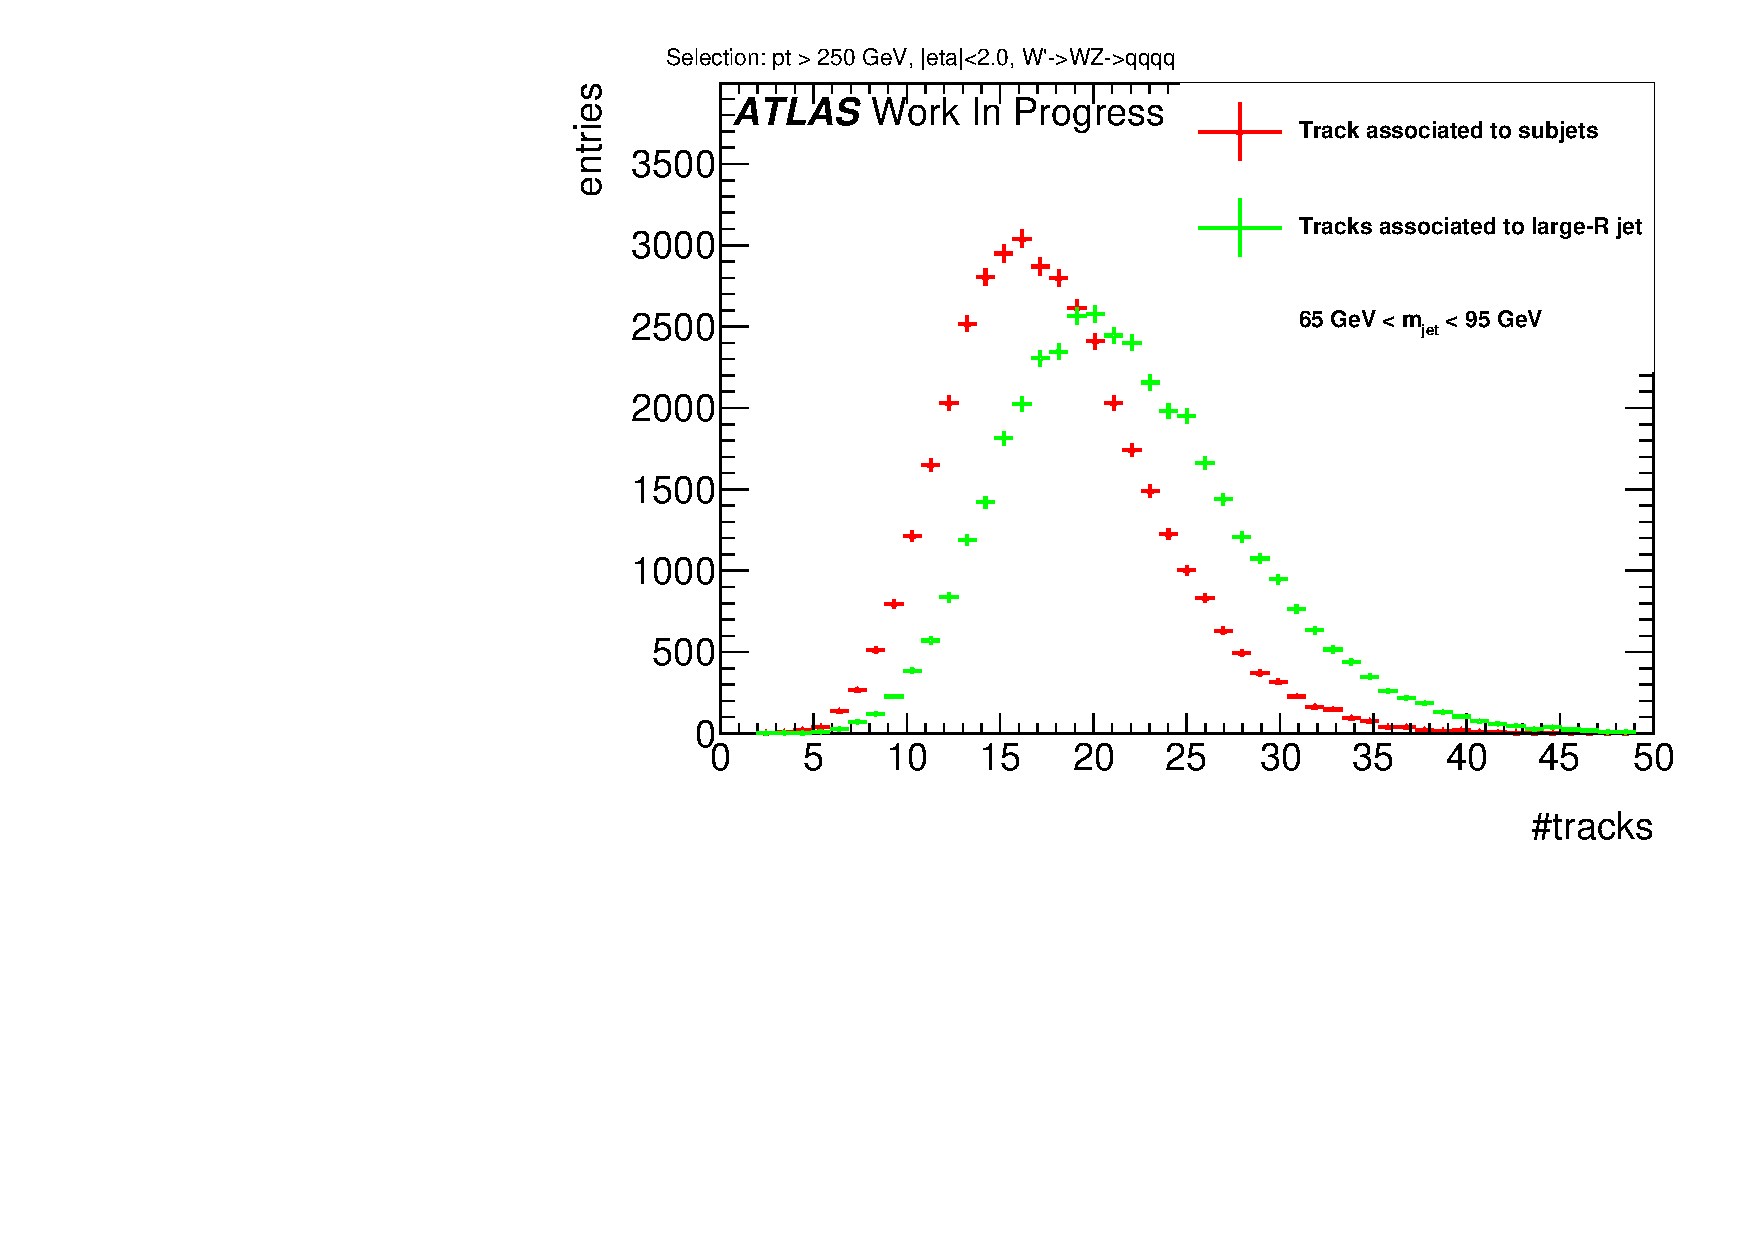
\includegraphics[width=0.5\textwidth]{sascha_input/plots/track_selection/h_customghost_number.pdf} \hspace{1mm}
	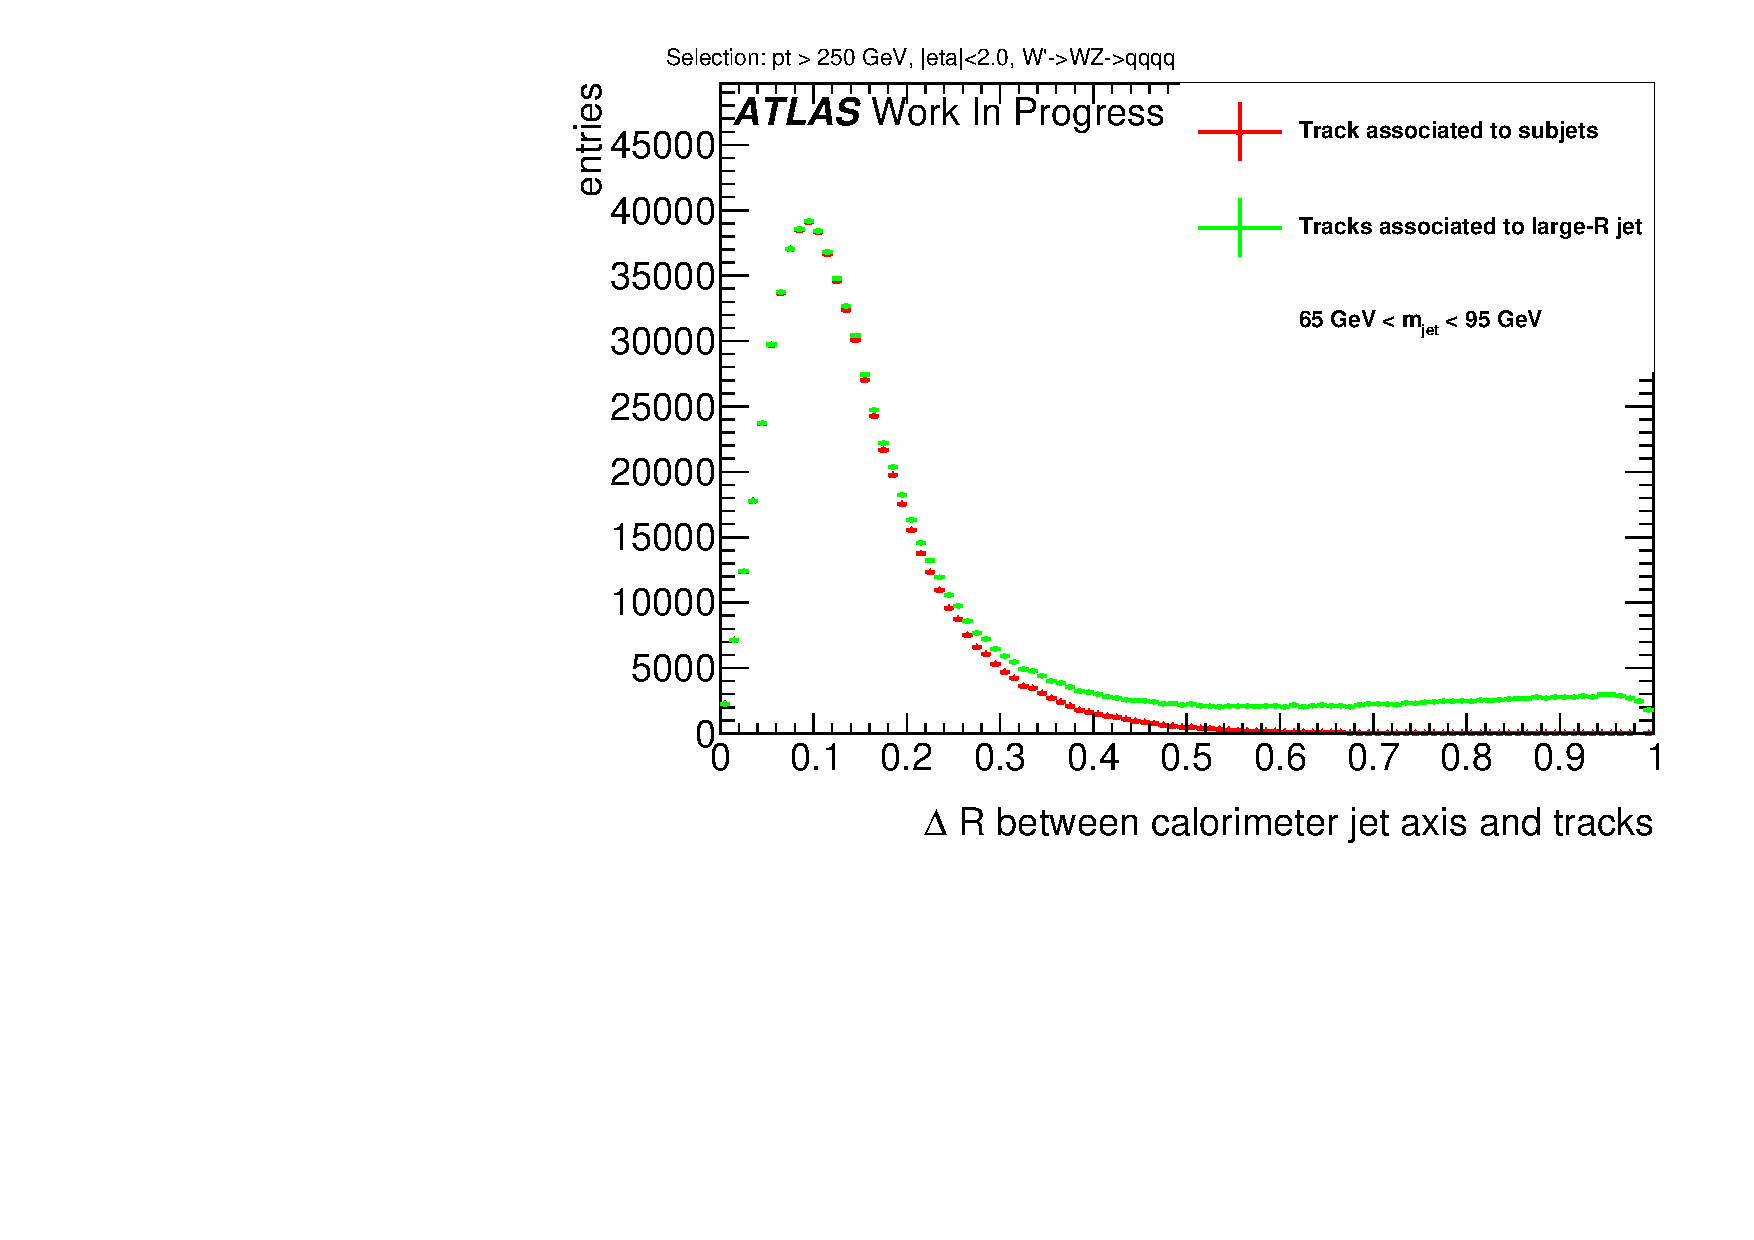
\includegraphics[width=0.5\textwidth]{sascha_input/plots/track_selection/h_customghost_dr.pdf}
\caption{\footnotesize{The number of tracks ghost associated to the large-R jet and to the sub-jets (left) and angular distance of associated tracks to the large-R calorimeter jet axis (right). Signal events were not reweighted at this step.}}\label{fig:delta_R}
\end{figure}

Figure \ref{fig:selection} shows the signal distributions of the C2/D2, and $\tau_{21}$, calculated with both selections of tracks for $W$ boson jets. The large $\Delta R$ to the jet axis of the differing tracks push the substructure variables to higher, more background like values. The broader distributions are a result of the variating nature of these tracks. C2 and D2 are more sensitive to tracks with a large $\Delta R$ to the jet axis, because the angular distance between all pairs and triples of tracks is considered, among tracks on possibly opposite ends of the large-R jet, whereas $\tau_{21}$uses distances to $k_\mathrm{T}$-WTA axes.
\begin{figure}
	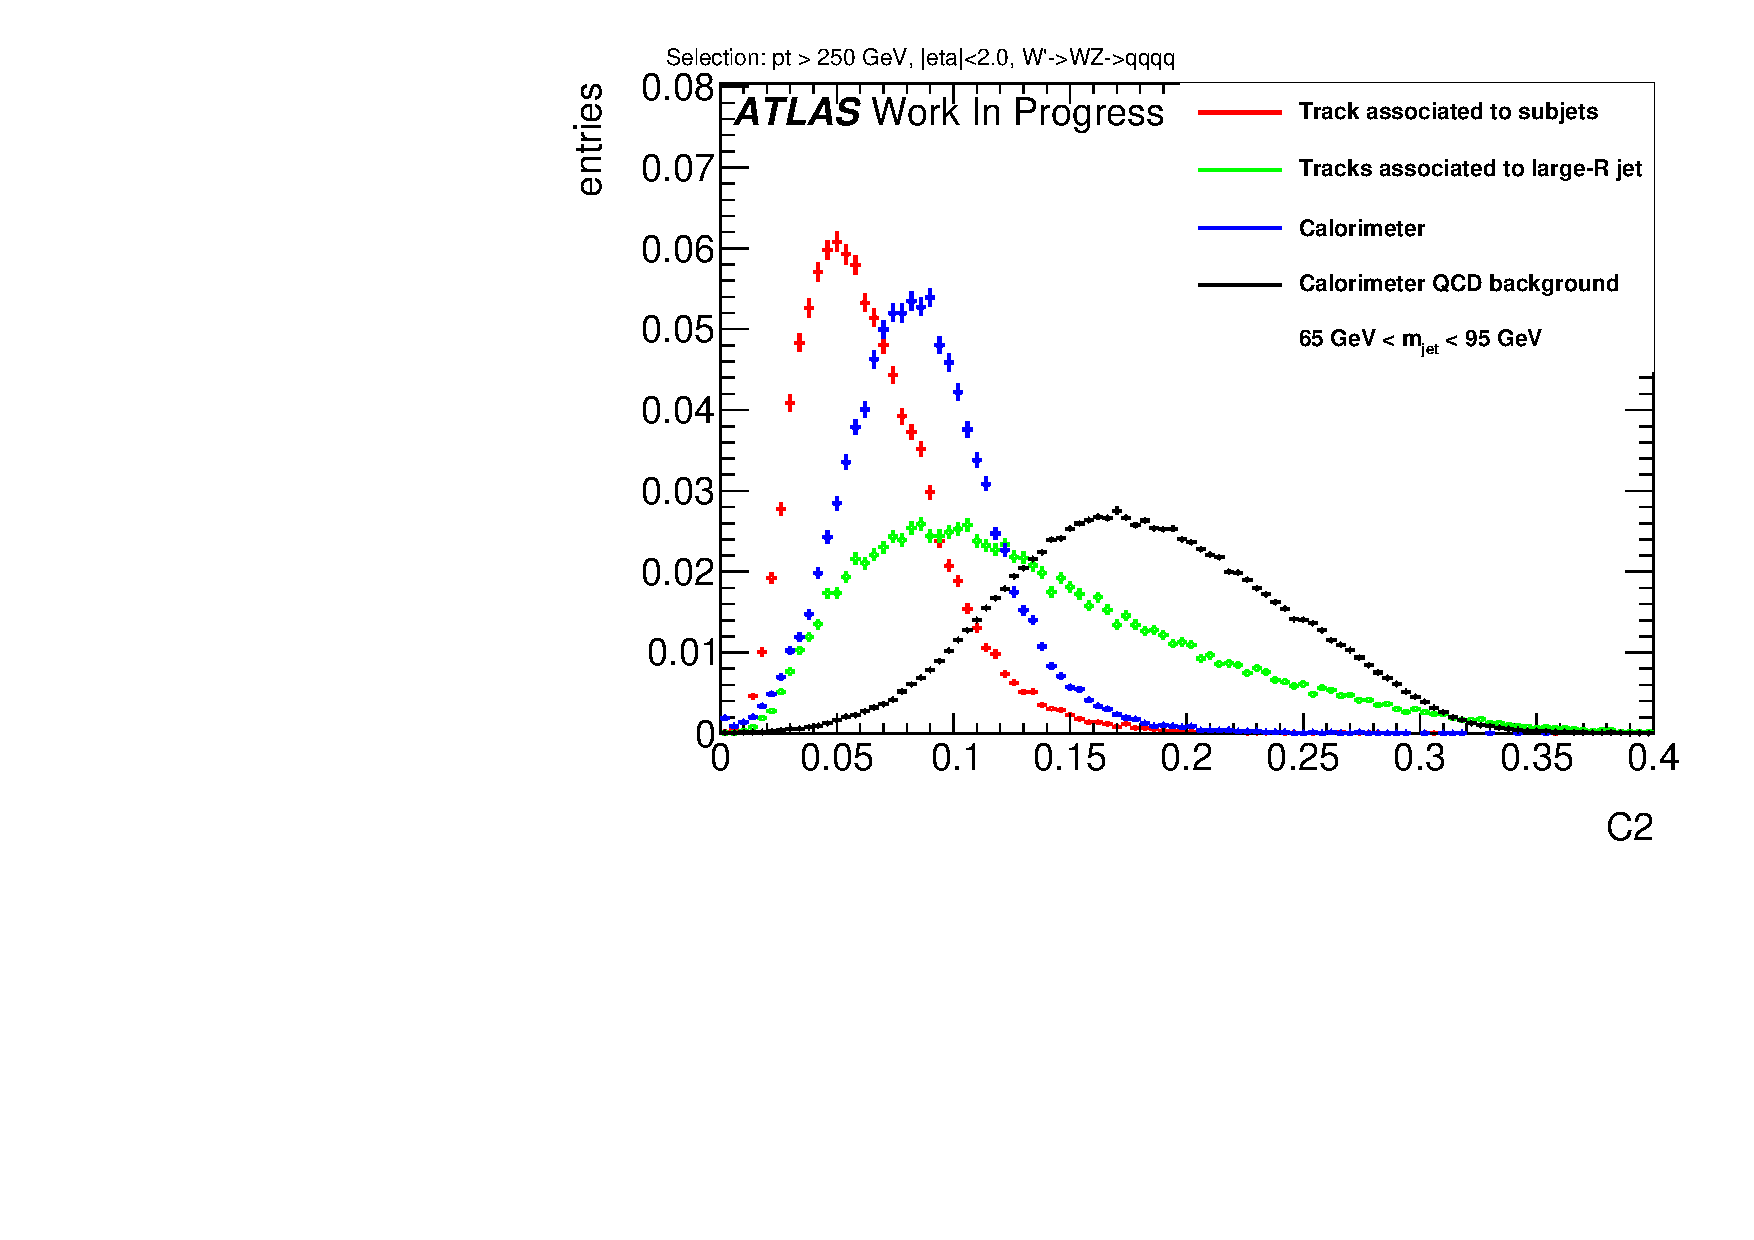
\includegraphics[width=0.45\textwidth]{sascha_input/plots/track_selection/h_ghost_sj_C2.pdf} \hspace{1mm}
	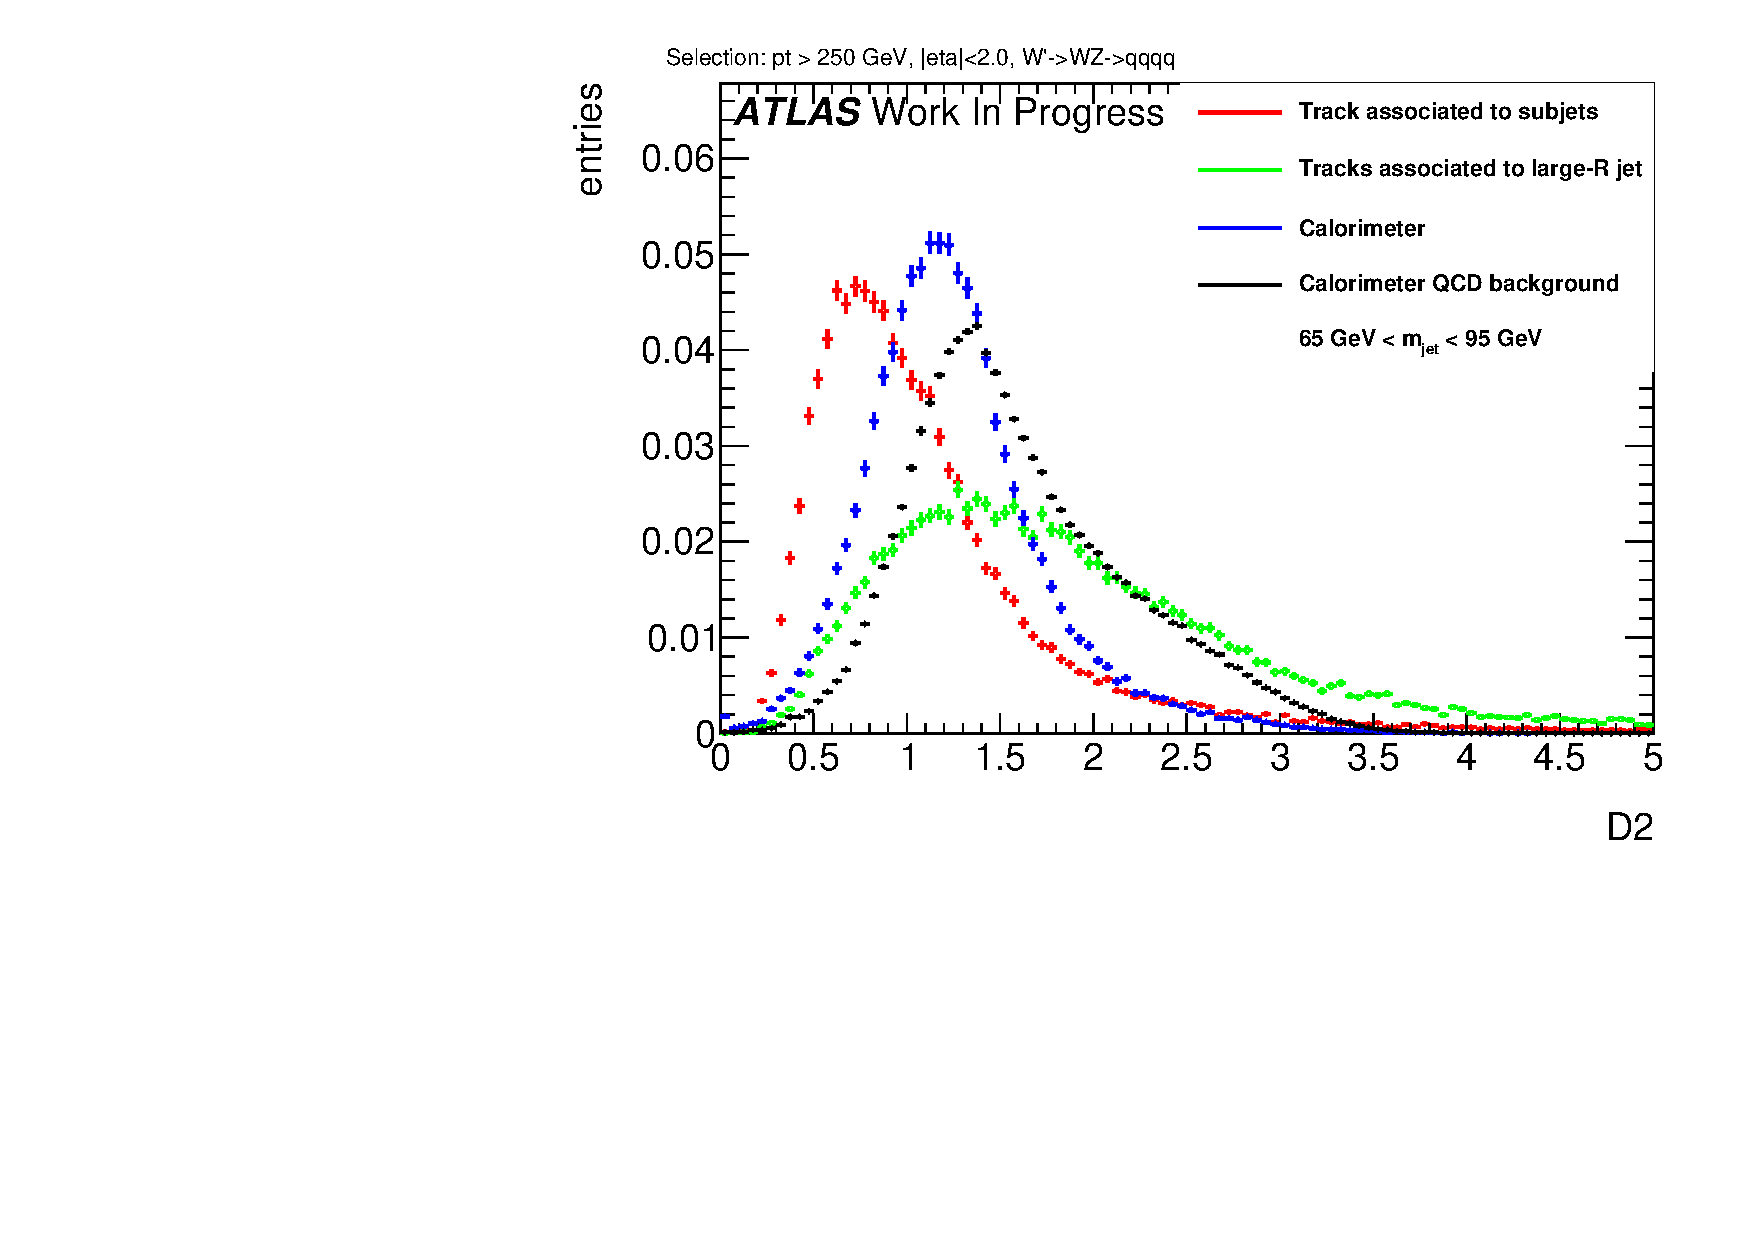
\includegraphics[width=0.45\textwidth]{sascha_input/plots/track_selection/h_ghost_sj_D2.pdf}
	\bigskip
	\centering
	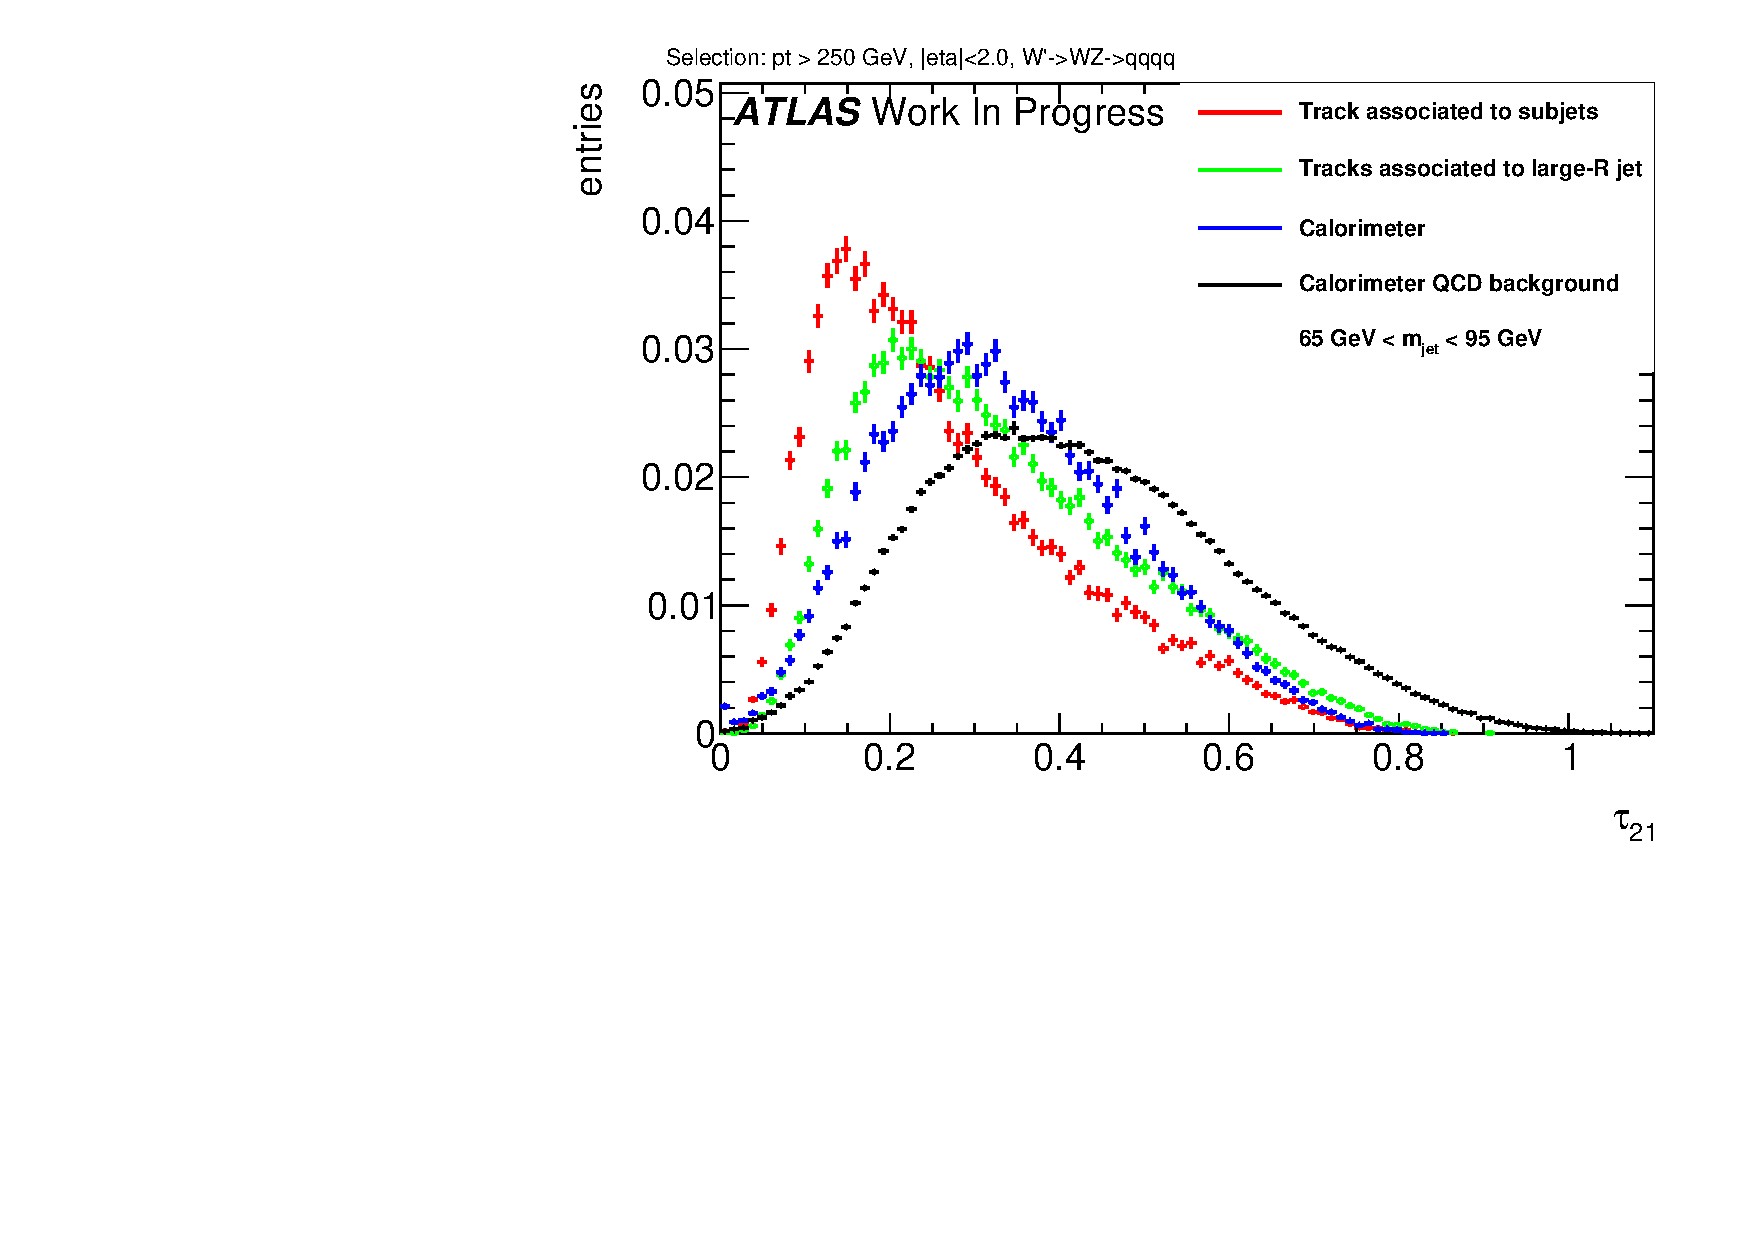
\includegraphics[width=0.45\textwidth]{sascha_input/plots/track_selection/h_ghost_sj_nSub21.pdf}
\caption{\footnotesize{Substructure variables (left) C2, (right) D2 and (below) $\tau_{21}$ calculateated with calorimeter clusters as well as tracks associated to sub-jets and to the large-R jet. Signal events were not reweighted at this step.}}\label{fig:selection}
\end{figure}
For comparison, the signal and background distributions for the variables calculated with calorimeter clusters are shown as well. It is possible to anticipate that the performance of variables calculated with tracks and assisted tracks is not worse than cluster base variables.
In contrast to the previously studied jet mass variable, ratios of ECF(N) and $\tau_N$ are rather energy scale independent and are found to not be as sensitive to the missing neutral fraction with un-assisted tracks.
Starting from this observations, the performance of substructure techniques is compared with the following objects as input:
\begin{itemize}
\item Calorimeter clusters, labeled 'calo'.
\item Tracks selected as described in Section \ref{subsec:ObsDef_Proc}, labeled 'tracks'.
\item The same collection of tracks, assisted as defined in Section \ref{subsec:ta_adapt}, labeled 'TAS'.
\end{itemize}
\label{sec:ECFnS}
%----------------------------------



%-------------------------------------------------------------------------------
\section{Conclusions}
\label{sec:conclusions}
%----------------------------------

%-------------------------------------------------------------------------------
\clearpage
\appendix
\part*{Appendix}
\addcontentsline{toc}{part}{Appendix}
%-------------------------------------------------------------------------------

In a paper, an appendix is used for technical details that would otherwise disturb the flow of the paper.
Such an appendix should be printed before the Bibliography.


%-------------------------------------------------------------------------------
% If you use biblatex and either biber or bibtex to process the bibliography
% just say \printbibliography here
\printbibliography
% If you want to use the traditional BibTeX you need to use the syntax below.
%\bibliographystyle{bibtex/bst/atlasBibStyleWoTitle}
%\bibliography{mydocument,bibtex/bib/ATLAS}
%-------------------------------------------------------------------------------

%-------------------------------------------------------------------------------
% Print the list of contributors to the analysis
% The argument gives the fraction of the text width used for the names
%-------------------------------------------------------------------------------
\clearpage
\PrintAtlasContribute{0.30}

%-------------------------------------------------------------------------------
\clearpage
\appendix
\part*{Auxiliary material}
\addcontentsline{toc}{part}{Auxiliary material}
%-------------------------------------------------------------------------------

In an ATLAS paper, auxiliary plots and tables that are supposed to be made public 
should be collected in an appendix that has the title \enquote{Auxiliary material}.
This appendix should be printed after the Bibliography.
At the end of the paper approval procedure, this information can be split into a separate document
-- see \texttt{atlas-auxmat.tex}.

In an ATLAS note, use the appendices to include all the technical details of your work
that are relevant for the ATLAS Collaboration only (e.g.\ dataset details, software release used).
This information should be printed after the Bibliography.

\end{document}
